\documentclass[varwidth=40cm]{standalone}
\usepackage{tikz}
\usepackage{style}

\begin{document}
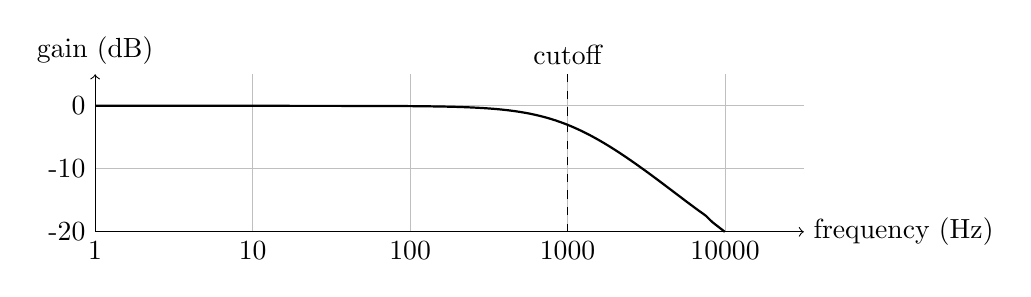
\begin{tikzpicture}[xscale=2,yscale=.08]
  \draw[lightgray] (0,0) -- (4.5,0);
  \draw[lightgray] (0,-10) -- (4.5,-10);
  \draw[lightgray] (0,-20) -- (4.5,-20);
  \draw[lightgray] (0,-20) -- (0,5);
  \draw[lightgray] (1,-20) -- (1,5);
  \draw[lightgray] (2,-20) -- (2,5);
  \draw[lightgray] (3,-20) -- (3,5);
  \draw[lightgray] (4,-20) -- (4,5);
  \draw[dashed] (3,-20) -- (3,5) node[above] {cutoff};
  \draw[->] (0,-20) -- (4.5,-20) node[right] {frequency (Hz)};
  \draw (0,-20) node[below] {1};
  \draw (1,-20) node[below] {10};
  \draw (2,-20) node[below] {100};
  \draw (3,-20) node[below] {1000};
  \draw (4,-20) node[below] {10000};
  \draw[->] (0,-20) -- (0,5) node[above] {gain (dB)};
  \draw (0,0) node[left] {0};
  \draw (0,-10) node[left] {-10};
  \draw (0,-20) node[left] {-20};
  \draw[thick,smooth,domain=0:4,samples=100] plot ({\x},{20*log10(1/sqrt(1+pow(pow(10,\x)/1000,2)))});
\end{tikzpicture}
\end{document}
